\documentclass[tikz,crop]{standalone}

\usepackage[T1]{fontenc}
\usepackage[tt=false,type1=true]{libertine}
\usepackage[varqu]{zi4}
\usepackage{newtxmath}
\usepackage[dvipsnames]{xcolor}
\usepackage{tikz,listings}
\usepackage{bbding}
\usetikzlibrary{arrows,fit,positioning,shadows,shapes,shapes.arrows}

\lstset{
    % backgroundcolor=\color{backcolour},
    % stringstyle=\color{codepurple},
    % commentstyle=\color{codegreen},
    keywordstyle=\bfseries\color{magenta},
    numberstyle=\tiny\color{codegray},
    basicstyle=\ttfamily\tiny,
    % captionpos=b,
    escapeinside={/@}{@/},
    % breakatwhitespace=false,
    % breaklines=true,
    % keepspaces=true,
    % numbers=left,
    % numbersep=5pt,
    % showspaces=false,
    % showstringspaces=false,
    % showtabs=false,
    % tabsize=2
}
\colorlet{ml-model-bg}{CornflowerBlue!10}
\colorlet{maru}{Green}
\colorlet{batsu}{OrangeRed!80}
\colorlet{tadashi}{Red}
\def\maru{{\color{maru}\CheckmarkBold}}
\def\batsu{{\color{batsu}\XSolidBold}}
\newbox\trainpy
\newbox\inputc
\newbox\outputc
\begin{document}

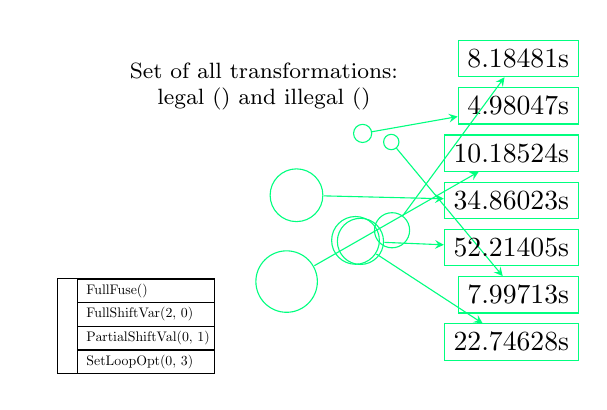
\begin{tikzpicture}

  %%% Begin Transformations %%%
  \node[
    % draw=black, densely dotted, rounded corners,
    text width=6cm, align=center,
    minimum height=4.5cm,
    text depth=3.4cm,
    anchor=north,
    font=\footnotesize,
    inner sep=0mm,
    % rectangle split, rectangle split parts=2,
  ] at (0, 2.8) {Set of all transformations: \\ legal ({\tiny\maru{}}) and illegal ({\tiny\batsu{}})};
  % XOXO
  \begin{scope}[xscale=2, yscale=1.5]
  \foreach [
    evaluate=\i as \xmaru using rand,
    evaluate=\i as \xbatsu using rand,
    evaluate=\i as \ymaru using rand,
    evaluate=\i as \ybatsu using rand,
    evaluate=\xmaru \ymaru as \smaru using (1.5-sqrt(\xmaru*\xmaru+\ymaru*\ymaru)),
    evaluate=\xbatsu \ybatsu as \sbatsu using (1.5-sqrt(\xbatsu*\xbatsu+\ybatsu*\ybatsu)),
    remember=\xmaru as \lxmaru (initially 0),
    remember=\ymaru as \lymaru (initially 0),
    ] \i in {1,2,...,50}{
    \node[scale=\sbatsu, opacity=1.2-\sbatsu] at (\xbatsu, \ybatsu) (batsu-\i) {\batsu};
    \node[scale=\smaru, opacity=1.2-\smaru] at (\xmaru, \ymaru) (maru-\i) {\maru};
  }

  \foreach [
    evaluate=\i as \xmaru using rand,
    evaluate=\i as \ymaru using rand,
    evaluate=\xmaru \ymaru as \smaru using (1.5-sqrt(\xmaru*\xmaru+\ymaru*\ymaru)),
    evaluate=\i as \time using abs(rand * rand) * 100,
    remember=\xmaru as \lxmaru (initially 0),
    remember=\ymaru as \lymaru (initially 0),
    ] \i in {1,2,...,7}{
    \node[draw, SpringGreen, circle, scale=2*\smaru] at (\xmaru, \ymaru) (ds-\i) {\color{SpringGreen}\CheckmarkBold};
    \node[draw=SpringGreen, anchor=east] at (2, 0.4*\i-1.2) (time-\i) {\time s};
    \draw[SpringGreen] (ds-\i) edge[-{stealth}] (time-\i);
  }
  \end{scope}
  %%% End Transformations %%%
  %%% Begin Samples %%%
  \path node [
    scale=0.5,
    draw=black,
    fill=white,
    rectangle split,
    rectangle split parts=4,
    rectangle split part align=left,
  ] at (-1.5cm, -1cm)
    (legend) {         \maru{}  FullFuse()
    \nodepart{two}     \maru{}  FullShiftVar(2, 0)
    \nodepart{three}   \maru{}  PartialShiftVal(0, 1)
    \nodepart{four}    \maru{}  SetLoopOpt(0, 3)
  }
  node [anchor=east, SpringGreen] at (legend.west) (leftlegend) {\CheckmarkBold}
  ;
  \node[draw, fit={(leftlegend) (legend)}, inner sep=0] {};
  %%% End Samples %%%
 
\end{tikzpicture}
\end{document}
